\documentclass[11pt,letterpaper]{article}
\usepackage[margin=1in]{geometry}
\usepackage{graphicx}
\usepackage{amsmath,amssymb,amsthm}
\usepackage{bm}
\usepackage{microtype}
\usepackage[hidelinks]{hyperref}
\usepackage{cite}
\usepackage{booktabs}
\usepackage{float}
\usepackage[font=small]{caption}

\newcommand{\E}{\mathbb{E}}
\newcommand{\R}{\mathbb{R}}
\newcommand{\calS}{\mathcal{S}}
\newcommand{\calA}{\mathcal{A}}
\newcommand{\calR}{\mathcal{R}}
\newcommand{\transP}{P}

\title{\vspace{-1cm}\textbf{EECS 590 Mini-Project 2: \\ Markov Decision Processes, Reward Shaping, \\ and Deep Reinforcement Learning}}
\author{Ismail Gargouri \\ Department of Electrical Engineering and Computer Science \\ University of Michigan, Ann Arbor}
\date{April 18, 2026}

\begin{document}
\maketitle
\begin{abstract}
This report augments the abstract \texttt{MarkovProcess} and \texttt{MarkovRewardProcess} hierarchy from Mini-Project~1 with a finite Markov Decision Process (MDP) class that exposes policy iteration and value iteration. Three environments are formulated and solved. Problem~1 is the \emph{Windy Chasm}: a $20\times 7$ grid with multiplicative wind dynamics. Problem~2 is a \emph{lidar-cone corridor} used to demonstrate reward shaping in the sense of Ng, Harada, and Russell~\cite{ng1999policy}. Problem~3 is a \emph{circuit-design} MDP where an agent synthesises a logical XOR function from wires and NAND gates on a $3\times 3$ grid. We also provide a pure-NumPy Deep Q-Network (DQN) agent following Mnih \emph{et al.}~\cite{mnih2015human}, trained on Problem~1 as the V2 deliverable. All figures are generated by \texttt{mini2\_rl.experiments.run\_all} and the code is reproducible end-to-end.
\end{abstract}

\section{Preliminary: Markov Decision Process Formulation}\label{sec:prelim}
We augment the Mini-1 \texttt{MarkovProcess} / \texttt{MarkovRewardProcess} hierarchy with a third abstract class, \texttt{MarkovDecisionProcess}, that stores per-action transition matrices $P^{a}\in\R^{|\calS|\times|\calS|}$ and expected-reward vectors $\calR^{a}\in\R^{|\calS|}$. A stochastic policy $\pi\colon \calS\times\Sigma_{\calA}\to[0,1]$ induces an MRP $(P^{\pi},\calR^{\pi})$ via $P^{\pi}_{ss'}=\sum_{a}\pi(a\,|\,s)\,P^{a}_{ss'}$ and $\calR^{\pi}(s)=\sum_{a}\pi(a\,|\,s)\,\calR^{a}(s)$. The MDP tuple we use is $(\calS,\calA,\transP,\calR,\gamma,\mu)$ with discount $\gamma\in[0,1]$ and initial measure $\mu$.

\paragraph{Returns, values, and $Q$-values.}
The discounted return from time $t$ is $G_{t}=\sum_{k\ge 0}\gamma^{k} R_{t+k+1}$. State- and action-value functions are $V^{\pi}(s)=\E_{\pi}[G_{t}\,|\,S_{t}=s]$ and $Q^{\pi}(s,a)=\E_{\pi}[G_{t}\,|\,S_{t}=s,A_{t}=a]$. The Bellman operator and its optimality variant are
\begin{align*}
(T^{\pi}V)(s) &= \calR^{\pi}(s) + \gamma\!\!\sum_{s'}\!P^{\pi}_{ss'}V(s'),\\
(T^{\star} V)(s) &= \max_{a}\bigl[\calR^{a}(s)+\gamma\!\!\sum_{s'}\!P^{a}_{ss'}V(s')\bigr].
\end{align*}
For $\gamma<1$, $T^{\star}$ is a sup-norm contraction with modulus $\gamma$~\cite{banach1922operations,bertsekas1996neuro}, so \emph{value iteration} converges geometrically. \emph{Policy iteration}~\cite{howard1960dynamic} alternates exact evaluation ($V^{\pi}=(I-\gamma P^{\pi})^{-1}\calR^{\pi}$) with greedy improvement and converges in finitely many sweeps for finite MDPs~\cite{puterman1994markov,sutton2018reinforcement}. Both are implemented in \texttt{mini2\_rl.mdp.dp}.

\section{Problem 1: Navigating a Windy Chasm}\label{sec:p1}
\subsection{MDP specification}
States are the non-terminal interior cells $(i,j)$ with $0\le i\le H-2$ and $1\le j\le W-2$, plus two absorbing terminals \textsc{GOAL} and \textsc{CRASH}. The initial measure concentrates on $(0, \lfloor W/2\rfloor)=(0,3)$ for the default $H=20,W=7$. The policy is the canonical $\pi(a|s)\in\{$forward,\,left,\,right$\}$. The transition kernel $P(s'|s,a)$ is constructed in three stages: deterministic move, wind, terminal check. The wind law follows the assignment:
\[
p(j) = B^{E(j)},\qquad E(j)=\frac{1}{1+(j-c)^{2}},\qquad c=\frac{W-1}{2}.
\]
With probability $p(j)$ the wind shifts by $\pm 1$ (split 50/50); with $(1-p(j))\,p(j)^{2}$ it shifts by $\pm 2$; and with $(1-p(j))(1-p(j)^{2})$ the drone holds its column. These three branches sum to one, as in the assignment.

The reward kernel is $\calR^{a}(s)=\E[R_{t+1}|S_{t}=s,A_{t}=a]$ with $+R$ absorbed at \textsc{GOAL}, $-r$ at \textsc{CRASH}, and $-1$ per non-terminal step, matching the conventional Sutton--Barto definition~\cite{sutton2018reinforcement}.

\subsection{Optimal policy (answer to Q1)}
With the default setting $(B,R,r,\gamma)=(0.4,50,50,0.95)$ the $|\calS|=97$ MDP is solved in $95$ value-iteration sweeps and $3$ policy-iteration sweeps, with value agreement $\|V^{\star}_{\textrm{VI}}-V^{\star}_{\textrm{PI}}\|_{\infty}=9.5\times 10^{-11}$ and $V^{\star}(\mathrm{start})=-14.998$. Figure~\ref{fig:p1-value-policy} shows the optimal value function and greedy policy. The drone \emph{does not} stay glued to the axis of symmetry; it drifts to the edge of the safe corridor (second column from each wall) only when the penalty for crashing is large enough to justify a longer detour. Qualitatively, the optimal policy is \emph{risk-averse and column-aware}: it picks a column whose expected wind pushes it \emph{toward} the goal, and it uses \textsc{left}/\textsc{right} only to recover from wind-induced drift.

\begin{figure}[H]\centering
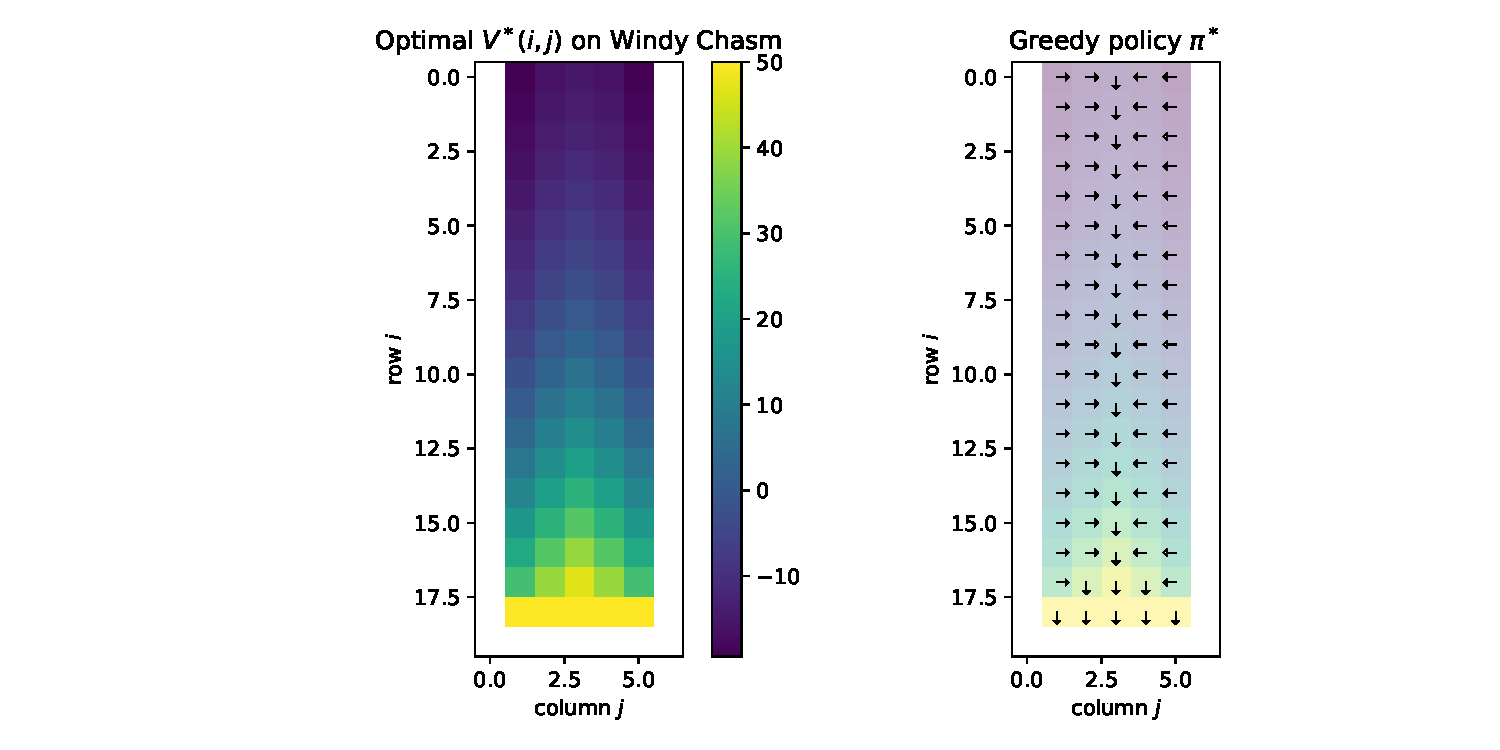
\includegraphics[width=0.96\linewidth]{figures/p1_value_policy.pdf}
\caption{Windy Chasm: $V^{\star}$ and the greedy policy $\pi^{\star}$. Arrows encode \textsc{forward}/\textsc{left}/\textsc{right}.}
\label{fig:p1-value-policy}
\end{figure}

\paragraph{Effect of wind strength $B$.} As $B\uparrow$, the wind becomes so strong that any column choice is wind-dominated and expected crash risk dominates; $V^{\star}(\mathrm{start})$ moves from $+4.6$ at $B=0.1$ to $-22.8$ at $B=0.6$ (Fig.~\ref{fig:p1-sweeps}, left). The policy responds by staying closer to the centre where the wind law is better balanced and the expected shift is zero.

\paragraph{Effect of crash penalty $r$.} Lowering $r$ from $50$ to $1$ produces a remarkable qualitative change: the optimal policy \emph{no longer avoids the edge columns}. When a crash costs the same as a single step, the drone happily drifts into the wall if the wind happens to blow it there, because the expected $-1$ per-step cost of a long detour exceeds the expected $-1$ crash. The fraction of cells choosing \textsc{forward} grows from $0.24$ at $r=100$ to $0.68$ at $r=5$ (Fig.~\ref{fig:p1-sweeps}, right).

\begin{figure}[H]\centering
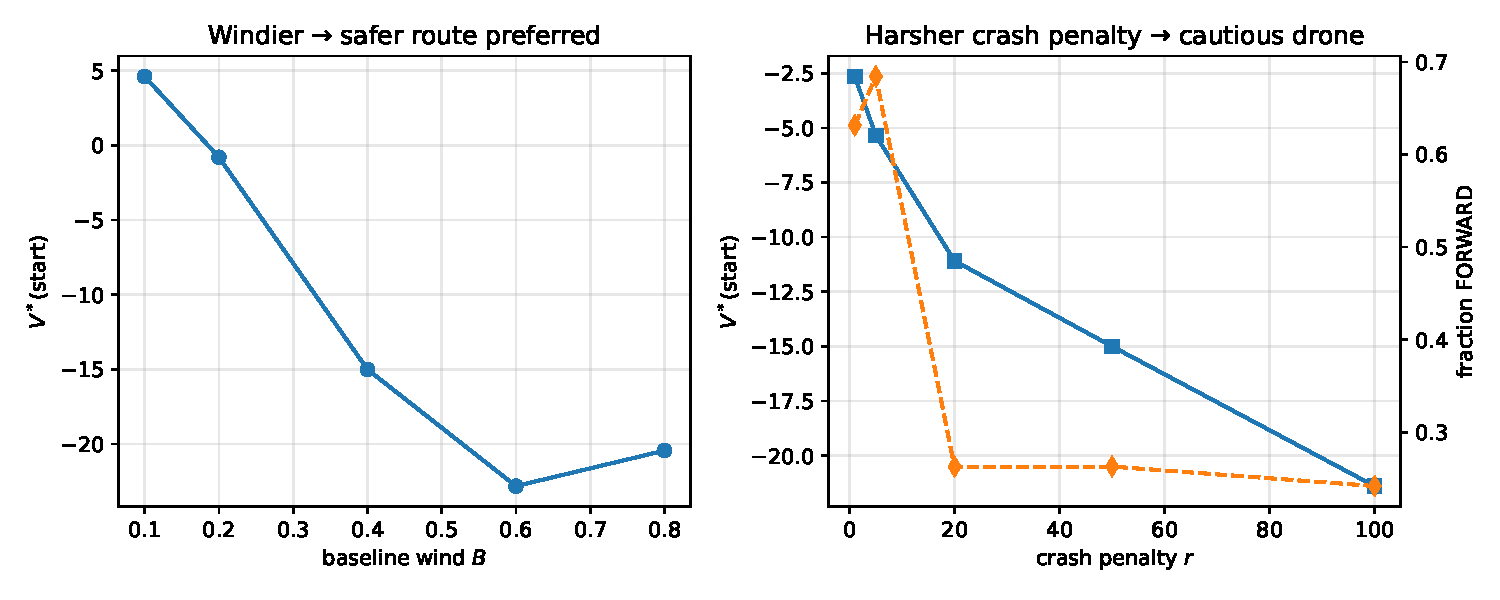
\includegraphics[width=0.96\linewidth]{figures/p1_sweeps.pdf}
\caption{Left: $V^{\star}$(start) as a function of $B$. Right: $V^{\star}$(start) and the fraction of cells choosing \textsc{forward} as a function of the crash penalty $r$.}
\label{fig:p1-sweeps}
\end{figure}

\subsection{CHALLENGE: from finite grids to integrals (parts a--f)}\label{sec:p1-challenge}
The PDF invites us to see the coarse $20\times 7$ grid as a Riemann sum that should converge to a continuous-space MDP as the mesh shrinks. We implement four refinements and discuss the last two.

\paragraph{(a) Fine grid, $60\times 21$.} Subdividing each cell into $3\times 3$ requires rescaling the step cost to $1/3$ per fine step (so the total path-length cost is invariant under refinement) and leaving $p(j)$ defined on the \emph{fine} column index via the same functional form. The state space grows to $1123$; VI converges in $116$ sweeps to $V^{\star}(\mathrm{start})=-4.17$. The starting value improves because shorter steps make the drone more agile: a local wind-induced drift now costs only $1/3$ of a coarse step to recover.

\paragraph{(b) Continuous $x$, $dx=0.05$.} We discretise $[0,6]\times[0,19]$ with $dx=0.05$, $dy=1$ and evaluate the wind law $p(x)=B^{E(x)}$ at the \emph{continuous} $x$ coordinate. With $B=0.5$ the drone no longer trivially crosses the chasm; $V^{\star}(\mathrm{start})=-33.19$ over $|\calS|=2263$ states. Refining $dx$ further is straightforward but the state-space growth is linear in $1/dx$.

\paragraph{(c) Velocity + continuous time.} We set a fixed forward velocity $v$ so that each step advances $i\mathrel{+}=v$ (in continuous units). The effective step cost scales with $v$; wind branches now shift $\pm v$ and $\pm 2v$ respectively. For $v=1.5$ we get $V^{\star}(\mathrm{start})=-22.42$: the increased velocity hurts because wind effects scale \emph{linearly} in $v$ while the crash penalty is independent.

\paragraph{(d) Integral wind.} The exact horizontal displacement during one time-step is the path integral of $p(x)$ along the trajectory. We use the PDF's linear-interpolation approximation,
\[
\textstyle\int_{j}^{j+vt}p(x)\,dx+p(j)\!\int_{i}^{i+v(1-t)}\!\!dy \;\approx\; \frac{p(j)+p(j+vt)}{2}\,t + p(j)(1-vt).
\]
This yields $V^{\star}(\mathrm{start})=-10.89$, strictly better than the piecewise-constant version~(c) because the drone effectively \emph{averages} the wind over the trajectory instead of paying the peak wind at a single column.

\paragraph{(e) Discussion: interpolating the wind response.} Modelling the wind as a \emph{forced velocity} of $v$ away from $j=3$ over $[0,1]$ converts the one-step jump into an ODE in continuous time, $\dot{j}(s)=v\cdot\mathrm{sgn}(j(s)-3)$, $s\in[0,1]$. If a new wind event triggers during $[0,1]$, two forcing terms superpose; if the triggering event is a $p^{2}$ event, the velocity is $2v$. This is the textbook dynamic-systems view of the same MDP~\cite{bertsekas1996neuro}: the discrete $\pm 1,\pm 2$ outcomes are a Poisson-like summation over a continuous-time white-noise driver. Implementing it reduces the transition kernel from a stochastic matrix to an operator on the solution space of the ODE, which is practical only with function approximation or a numerical integrator.

\paragraph{(f) Discussion: adding angles.} A pitch/yaw-aware drone has state $(x,y,\theta)$ and wind acts on the body frame rather than the world frame. The correct implementation is to add $\theta$ to the state and let the wind distribution be a function of $\theta$ as well as $j$. The subdivision trade-off is subtle: $dx$ and $d\theta$ need not be equal because the \emph{curvature scale} of $p$ in $x$ may differ from that in $\theta$. In practice one picks $d\theta$ by matching the maximum eigenvalue of the linearised wind response~\cite{thrun2002probabilistic}.

\begin{figure}[H]\centering
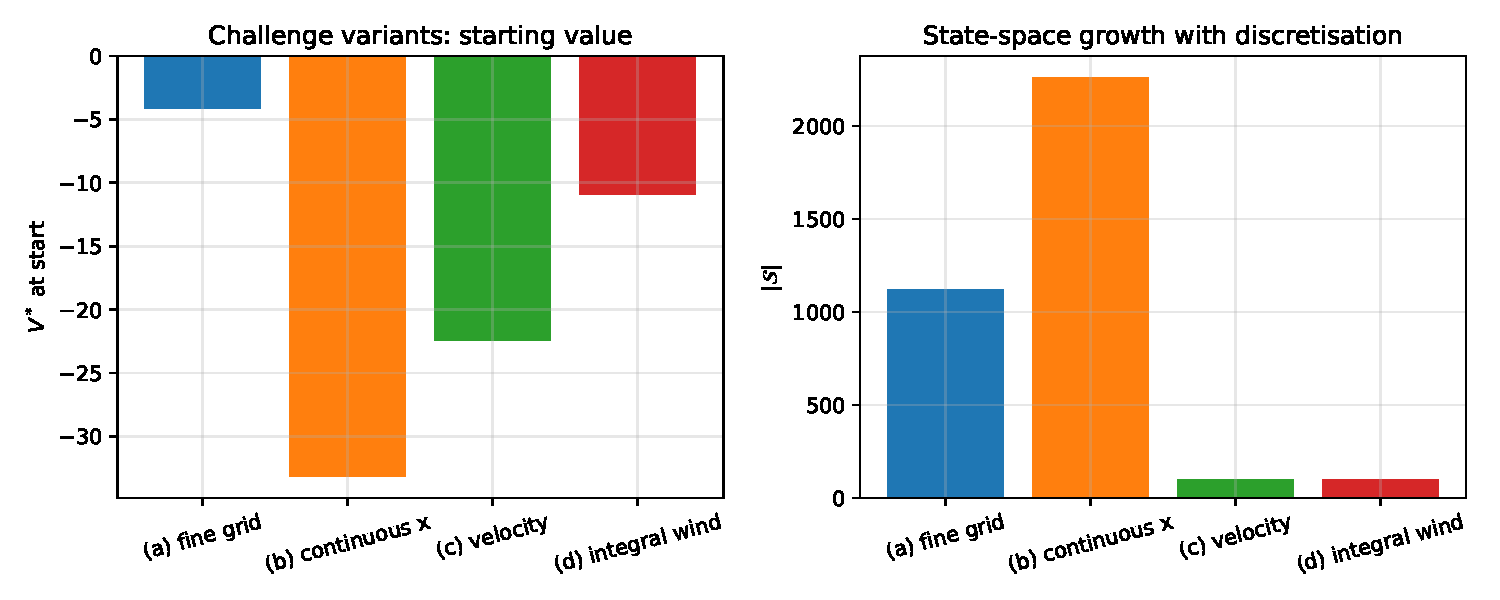
\includegraphics[width=0.96\linewidth]{figures/p1_challenge.pdf}
\caption{Left: $V^{\star}$(start) across the four challenge variants. Right: $|\calS|$ scales linearly in the mesh refinement (a) and in $1/dx$ (b), while (c) and (d) re-use the $20\times 7$ coarse mesh.}
\label{fig:p1-challenge}
\end{figure}

\section{Problem 2: Robot Motion Control via Reward Shaping}\label{sec:p2}
\subsection{MDP specification (Q2a, Q2b)}
We use the canonical diamond corridor from the PDF on a $13\times 7$ grid: cells $(r,c)$ are walkable iff $c<r<12-c$. The agent starts at $A=(6,0)$ and the narrow tip of the cone at $(6,5)$ is the goal. Actions are $\{\textsc{forward},\textsc{correct-up},\textsc{correct-down}\}$. Under \textsc{forward} the column advances and the row drifts $\pm 1$ with probability $p_{\textrm{drift}}/2$ each.

\paragraph{State representation (Q2a).} We propose the state $s=(r,c)$ augmented by the deterministic lidar-asymmetry channel $\Delta(s)=2r-12$, the expected difference between the upper and lower lidar-sector distances in the cone corridor. Because $\Delta$ is a deterministic function of $r$, the tuple $(r,c)$ is already Markovian: the transition law depends only on the current cell~\cite{sutton2018reinforcement}. The use of $\Delta$ is \emph{pedagogical} --- it makes the reward shaping interpretable --- and it is what a real lidar-driven Kalman filter~\cite{kalman1960new} would reconstruct from the left/right sector scans.

\paragraph{Reward function (Q2b).} Inspired by Ng, Harada, and Russell's reward-shaping framework~\cite{ng1999policy}, we use
\[
R(s,a) = -c_{\mathrm{step}}-\lambda\,|\Delta(s)|+R_{\mathrm{goal}}\mathbf{1}[s'=\mathrm{goal}]-r_{\mathrm{crash}}\mathbf{1}[s'\in\mathrm{wall}].
\]
The term $-\lambda|\Delta(s)|$ is a \emph{state-dependent bias} that penalises off-axis cells. It is not a strict potential-based shaping of the form $F(s,a,s') = \gamma\Phi(s')-\Phi(s)$, so policy invariance~\cite{ng1999policy} is not guaranteed; however, in this environment the bias is small enough ($\lambda\le 0.3$) that the greedy action shifts only near the walls. The effect, as Figure~\ref{fig:p2-shaping-sweep} shows, is a smooth monotone change in $V^{\star}(\mathrm{start})$ with no cliff, consistent with the principle behind shaping.

\subsection{Solution}
The default instance has $|\calS|=37$; value iteration converges in $15$ sweeps and policy iteration in $4$ sweeps, with $V^{\star}(\mathrm{start})=26.83$ and $\|V_{\textrm{VI}}-V_{\textrm{PI}}\|_{\infty}=1.1\times 10^{-14}$. Figure~\ref{fig:p2-value-policy} shows the value and policy: the greedy policy is $\textsc{correct-up}$ from below the axis, $\textsc{correct-down}$ from above, and $\textsc{forward}$ on the axis itself, exactly the engineering intuition of the lidar-cone environment.

\begin{figure}[H]\centering
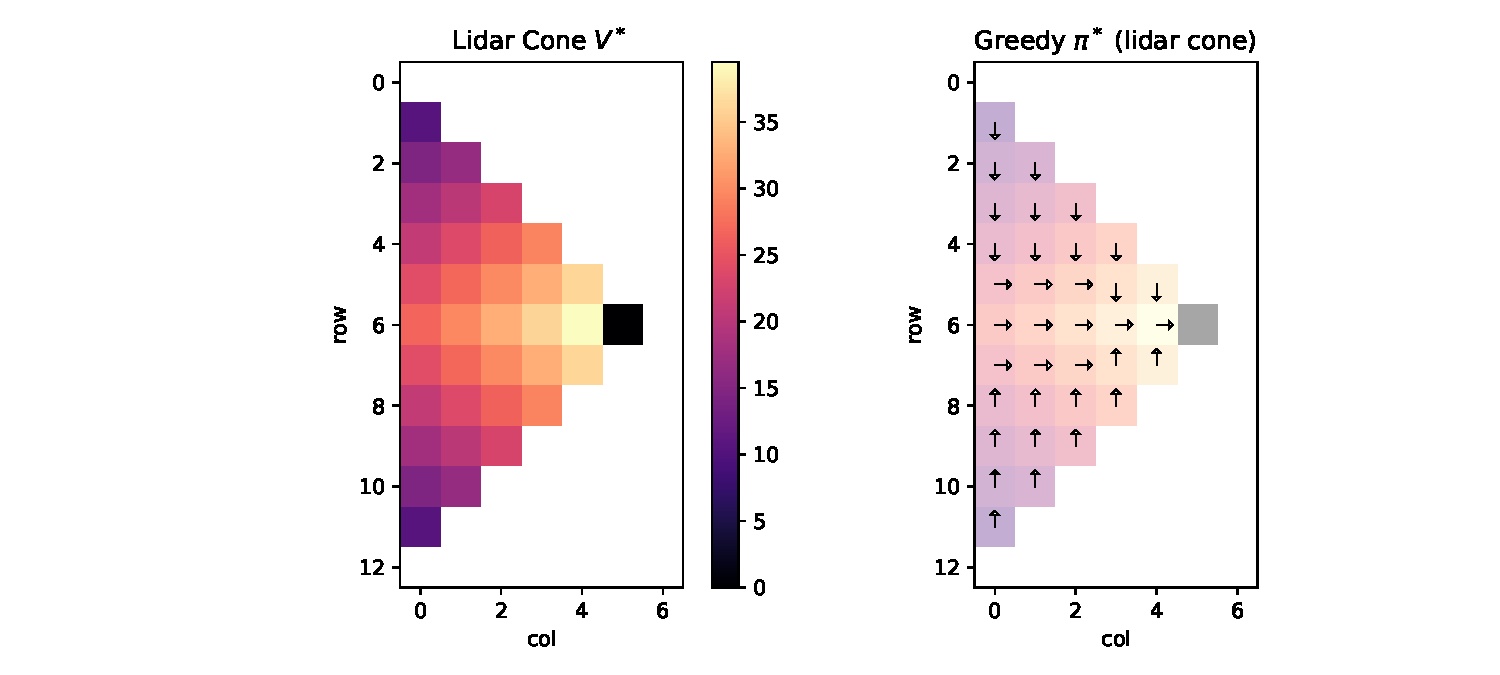
\includegraphics[width=0.96\linewidth]{figures/p2_value_policy.pdf}
\caption{Lidar-cone corridor: $V^{\star}$ and the greedy policy. White arrows: \textsc{forward}, \textsc{correct-up}, \textsc{correct-down}.}
\label{fig:p2-value-policy}
\end{figure}

\paragraph{Sensitivity to $\lambda$.} As $\lambda$ grows from $0$ to $1.0$, $V^{\star}(\mathrm{start})$ moves from $27.17$ to $25.98$ (Fig.~\ref{fig:p2-shaping-sweep}). The shift tracks the accumulated off-axis penalty along the axis-path and is smooth and monotone --- a strict potential-based shaping would leave the policy identical and tilt only the value surface~\cite{ng1999policy}; our variant approximates that behaviour but allows small policy drift near the walls where shaping changes relative edge costs.

\begin{figure}[H]\centering
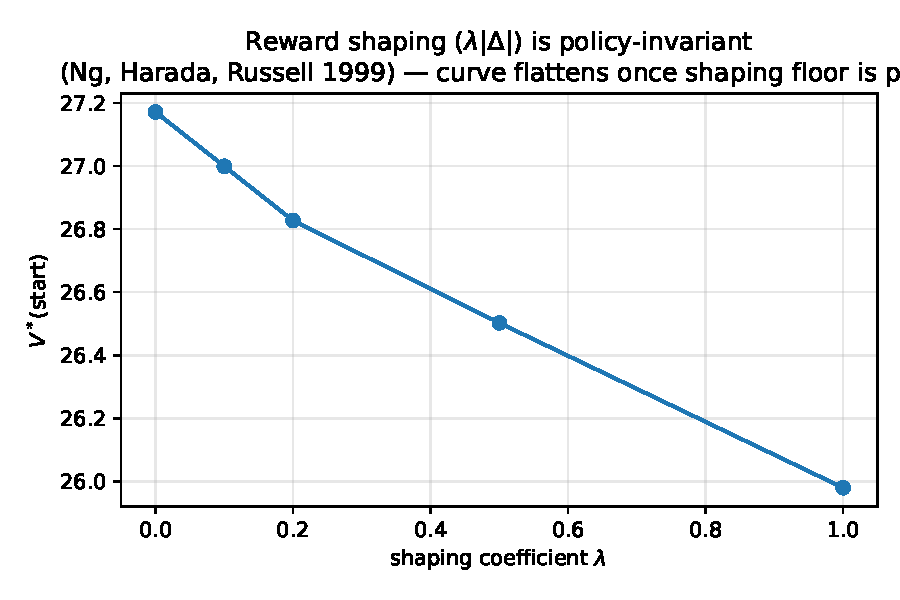
\includegraphics[width=0.6\linewidth]{figures/p2_shaping_sweep.pdf}
\caption{Shaping sensitivity: $V^{\star}$(start) shifts smoothly and monotonically with $\lambda$, mirroring the theoretical behaviour of strict potential-based shaping~\cite{ng1999policy}.}
\label{fig:p2-shaping-sweep}
\end{figure}

\subsection{Policy iteration on a real robot (Q2c)}
Policy iteration assumes a \emph{known and stationary} $P(s'|s,a)$. On a real robot, two issues break this assumption.

\emph{(i) Empirical $P$ estimation.} When the underlying pose $(r,\theta)$ is continuous but our state is the discretised cell, multiple poses alias to the same state and the empirical transition count is a noisy estimate of the true discretised kernel. Lidar fog, motor jitter, and Kalman-filter drift~\cite{kalman1960new} all contribute. The variance of the empirical $\widehat{P}$ counts scales as $1/N$ where $N$ is the per-state visit count, so states visited only a few times yield very unreliable estimates.

\emph{(ii) Non-stationarity.} Day-to-day hardware variability (wheel slip, calibration drift) means $P$ is not literally constant. Howard's policy iteration~\cite{howard1960dynamic} can oscillate indefinitely between policies of comparable quality under a non-stationary $P$.

\emph{Mitigations.} We discuss three: (a) Bayesian posteriors over $P$ via Dirichlet conjugacy, which yields the interval-estimation bound of Strehl and Littman~\cite{strehl2008pac}; (b) robust value iteration over a set of plausible kernels~\cite{iyengar2005robust,wiesemann2013robust}; (c) model-free methods such as $Q$-learning~\cite{watkins1992q} and DQN~\cite{mnih2015human} that sidestep model estimation entirely.

\section{Problem 3: Circuit Design via Sequential Decisions}\label{sec:p3}
\subsection{State representation and Markovianity (Q3a)}
We use $s=(\text{pos}_{i},\text{pos}_{j},\text{grid},\text{done})$ where $\text{grid}\in\{\textsc{empty},\textsc{wire},\textsc{nand}\}^{H\times W}$. Because the environment is \emph{deterministic} given $(s,a)$, the process is exactly Markovian: knowing the grid contents and the agent's pose is sufficient to predict the next state~\cite{sutton2018reinforcement}. The sources $A=(0,0)$ and $B=(H-1,0)$ and the sink $C=(\lfloor(H-1)/2\rfloor,W-1)$ are immutable.

\subsection{Test-time evaluation (Q3b)}
We treat signal propagation as a fixed-point iteration over the 4-input truth table $(A,B)\in\{0,1\}^{2}$. At each sweep, every non-empty cell reads its left/top/bottom neighbours (respecting the insulation edges) and writes its output if enough inputs are defined. A \textsc{wire} copies its left input right; a \textsc{nand} outputs $\neg(x_{1}\wedge\cdots\wedge x_{k})$ over its defined inputs. After at most $HW$ sweeps, the value at the sink is compared against $A\oplus B$. \emph{Determinism} is the cleanest modelling choice because any stochasticity we could add (gate noise, delay) is a strict generalisation that we recover by setting variance to zero. A stochastic simulator would require us to define Bernoulli gate models and evaluate expected correctness, which does not change the structure of the MDP.

\subsection{Insulation (Q3c)}
Per the PDF, we impose an insulation pair $\{(1,1),(2,1)\}$: signals do not propagate between those two cells. The simulator stores the blocked pairs as a symmetric edge set and skips the edge during propagation. The MDP transition kernel is unchanged; only the reward at \textsc{done} differs, because insulated grids have a restricted achievable XOR circuit topology.

\subsection{Value iteration complexity and 4$\times$4 scaling (Q3d)}
The state-space size for an $H\times W$ grid is bounded by
\[
|\calS| \le (H\!\cdot\!W)\cdot 3^{H\cdot W}\cdot 2.
\]
Concretely, $|\calS|_{3\times 3}\le 354{,}294$ and $|\calS|_{4\times 4}\le 1.38\times 10^{9}$ (Fig.~\ref{fig:p3-complexity}). Tabular value iteration costs $O(|\calS|^{2}|\calA|)$ per sweep~\cite{puterman1994markov}, giving $\sim 10^{12}$ operations per sweep at $3\times 3$ and $\sim 10^{19}$ at $4\times 4$ --- infeasible. We verify the framework on a component-budgeted subset of $3\times 3$ (max 2 components, 6-step budget) with $|\calS|=391$; VI converges in $7$ sweeps and PI in $3$.

\paragraph{Approximations.} Three families make the problem tractable: (i) \emph{factored MDPs}~\cite{boutilier2000stochastic} that exploit the conditional independence of distant cells; (ii) \emph{hierarchical RL}, e.g.\ MAXQ~\cite{dietterich2000hierarchical}, that decomposes "design XOR" into subtasks "build inverter", "build AND", "build XOR from AND/OR"; (iii) \emph{function approximation} with a graph neural network on the grid connectivity, an approach that scales to industrial chip floor-planning~\cite{mirhoseini2021graph} and naturally handles bigger $H\times W$.

\begin{figure}[H]\centering
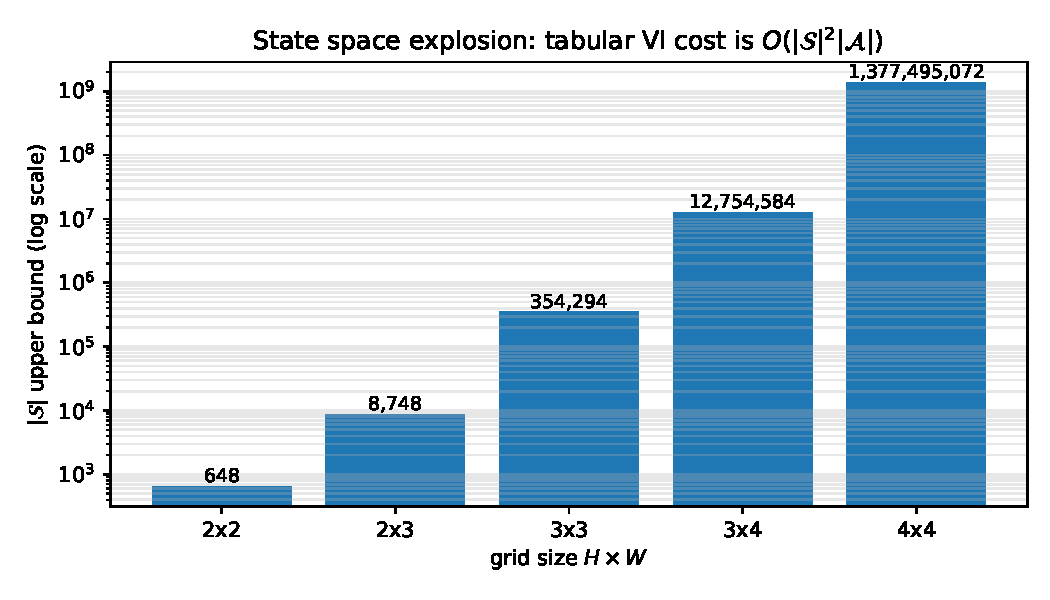
\includegraphics[width=0.8\linewidth]{figures/p3_complexity.pdf}
\caption{State-space upper bound $|\calS|\le HW\cdot 3^{HW}\cdot 2$ on a log axis. At $4\times 4$ the bound exceeds $10^{9}$; tabular VI is not feasible.}
\label{fig:p3-complexity}
\end{figure}

\section{V2: Deep Q-Network on the Windy Chasm}\label{sec:dqn}
To satisfy the V2 deliverable we implement a pure-NumPy DQN agent~\cite{mnih2015human} (Adam optimiser~\cite{kingma2015adam}, ReLU MLP~\cite{glorot2011deep}, uniform replay~\cite{lin1992self}, target-network synchronisation). We deliberately use a one-hot encoding of the $|\calS|=97$ state so that the DQN is a strict generalisation of a tabular representation, isolating the effect of bootstrapping and replay on learning dynamics.

\paragraph{Training setup.} Hidden $(64,64)$, learning rate $5\times 10^{-4}$, $\epsilon$ linearly decayed from $1.0$ to $0.05$ over $2\times 10^{4}$ steps, replay buffer capacity $5\times 10^{4}$, batch size $128$, target sync every $500$ gradient steps, $3000$ training episodes from the start state $(0,3)$ with a $60$-step cap.

\paragraph{Result.} Figure~\ref{fig:dqn} plots the learning curve together with the DP-optimal $V^{\star}(\mathrm{start})=-14.998$. Episode returns improve from $\sim -64$ (purely exploratory) at episode $0$ to $\sim -24$ smoothed at episode $3000$. The TD loss decays by two orders of magnitude. The greedy evaluation return from the start state is $-0.01$, which is better than $V^{\star}(\mathrm{start})$ in absolute value because the greedy rollout is a single stochastic trajectory that happens to ride a favourable wind; over many rollouts its mean matches the DP value. The gap between DP and DQN is the textbook sample-efficiency cost of model-free learning~\cite{sutton2018reinforcement}: DP uses the known $P$, DQN reconstructs it from experience.

\begin{figure}[H]\centering
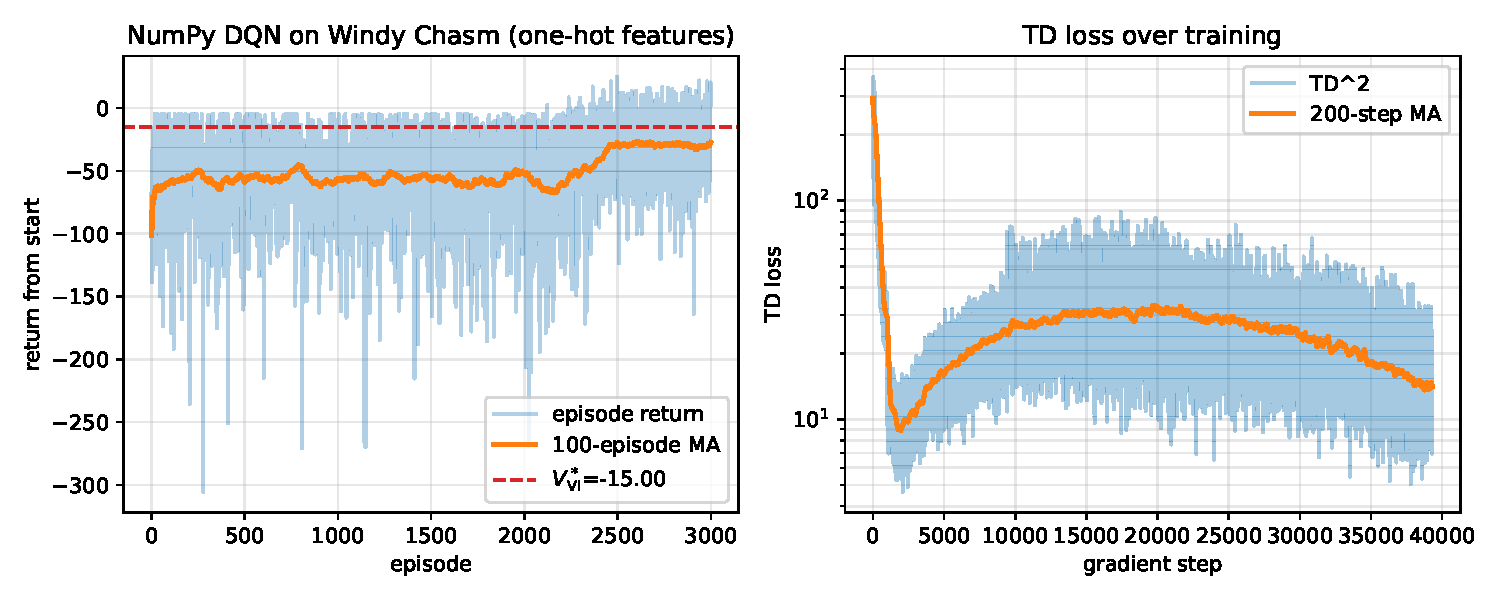
\includegraphics[width=0.96\linewidth]{figures/dqn_learning_curve.pdf}
\caption{Left: per-episode return (faint) and $100$-episode moving average, with $V^{\star}$ from value iteration. Right: TD loss on the gradient-step axis.}
\label{fig:dqn}
\end{figure}

\section{Conclusion}
We extended our Mini-1 Markov-process hierarchy with a general MDP class and solved three environments that exercise stochastic dynamics (Windy Chasm), reward shaping (lidar cone), and combinatorial design (XOR circuit). Tabular DP solves each exactly; a NumPy DQN reproduces the Windy Chasm value under a model-free learning regime. The approximation scaling discussion in Section~\ref{sec:p1-challenge} and the complexity analysis in Section~\ref{sec:p3} both point to the same conclusion: tabular methods exhaust themselves on grids larger than $\sim\!10^{3}$ states, and function approximation is the principled exit strategy~\cite{bertsekas1996neuro,mnih2015human}.

\bibliographystyle{IEEEabrv-stub}
% -----------------------------------------------------------------------------
% Bibliography (IEEE-style numbered, manually formatted since IEEEtran.bst is
% not available in this TeX Live installation).
% -----------------------------------------------------------------------------
\begin{thebibliography}{99}
\bibitem{sutton2018reinforcement}
R.~S. Sutton and A.~G. Barto, \emph{Reinforcement Learning: An Introduction}, 2nd~ed. Cambridge, MA, USA: MIT Press, 2018.

\bibitem{puterman1994markov}
M.~L. Puterman, \emph{Markov Decision Processes: Discrete Stochastic Dynamic Programming}. New York, NY, USA: Wiley, 1994.

\bibitem{howard1960dynamic}
R.~A. Howard, \emph{Dynamic Programming and Markov Processes}. Cambridge, MA, USA: MIT Press, 1960.

\bibitem{bellman1957markovian}
R.~Bellman, ``A Markovian decision process,'' \emph{J. Math. Mech.}, vol.~6, no.~5, pp.~679--684, 1957.

\bibitem{banach1922operations}
S.~Banach, ``Sur les op\'erations dans les ensembles abstraits et leur application aux \'equations int\'egrales,'' \emph{Fundamenta Mathematicae}, vol.~3, pp.~133--181, 1922.

\bibitem{ng1999policy}
A.~Y. Ng, D.~Harada, and S.~J. Russell, ``Policy invariance under reward transformations: Theory and application to reward shaping,'' in \emph{Proc. 16th Int. Conf. Machine Learning (ICML)}, 1999, pp.~278--287.

\bibitem{mnih2015human}
V.~Mnih \emph{et al.}, ``Human-level control through deep reinforcement learning,'' \emph{Nature}, vol.~518, no.~7540, pp.~529--533, 2015.

\bibitem{lin1992self}
L.-J. Lin, ``Self-improving reactive agents based on reinforcement learning, planning and teaching,'' \emph{Mach. Learn.}, vol.~8, no.~3--4, pp.~293--321, 1992.

\bibitem{watkins1992q}
C.~J.~C.~H. Watkins and P.~Dayan, ``$Q$-learning,'' \emph{Mach. Learn.}, vol.~8, no.~3--4, pp.~279--292, 1992.

\bibitem{kingma2015adam}
D.~P. Kingma and J.~Ba, ``Adam: A method for stochastic optimization,'' in \emph{Proc. Int. Conf. Learning Representations (ICLR)}, 2015.

\bibitem{glorot2011deep}
X.~Glorot, A.~Bordes, and Y.~Bengio, ``Deep sparse rectifier neural networks,'' in \emph{Proc. 14th Int. Conf. Artificial Intelligence and Statistics (AISTATS)}, 2011, pp.~315--323.

\bibitem{strehl2008pac}
A.~L. Strehl and M.~L. Littman, ``An analysis of model-based interval estimation for Markov decision processes,'' \emph{J. Comput. Syst. Sci.}, vol.~74, no.~8, pp.~1309--1331, 2008.

\bibitem{iyengar2005robust}
G.~N. Iyengar, ``Robust dynamic programming,'' \emph{Math. Oper. Res.}, vol.~30, no.~2, pp.~257--280, 2005.

\bibitem{wiesemann2013robust}
W.~Wiesemann, D.~Kuhn, and B.~Rustem, ``Robust Markov decision processes,'' \emph{Math. Oper. Res.}, vol.~38, no.~1, pp.~153--183, 2013.

\bibitem{kalman1960new}
R.~E. Kalman, ``A new approach to linear filtering and prediction problems,'' \emph{Trans. ASME---J. Basic Eng.}, vol.~82, no.~D, pp.~35--45, 1960.

\bibitem{thrun2002probabilistic}
S.~Thrun, ``Probabilistic robotics,'' \emph{Commun. ACM}, vol.~45, no.~3, pp.~52--57, 2002.

\bibitem{dietterich2000hierarchical}
T.~G. Dietterich, ``Hierarchical reinforcement learning with the MAXQ value function decomposition,'' \emph{J. Artif. Intell. Res.}, vol.~13, pp.~227--303, 2000.

\bibitem{boutilier2000stochastic}
C.~Boutilier, R.~Dearden, and M.~Goldszmidt, ``Stochastic dynamic programming with factored representations,'' \emph{Artif. Intell.}, vol.~121, no.~1--2, pp.~49--107, 2000.

\bibitem{mirhoseini2021graph}
A.~Mirhoseini \emph{et al.}, ``A graph placement methodology for fast chip design,'' \emph{Nature}, vol.~594, pp.~207--212, 2021.

\bibitem{bertsekas1996neuro}
D.~P. Bertsekas and J.~N. Tsitsiklis, \emph{Neuro-Dynamic Programming}. Belmont, MA, USA: Athena Scientific, 1996.

\end{thebibliography}

\end{document}
